\clearpage

\subsection{Testen}
\label{sec:Testen}

\subsubsection{Klassifizierung von Testverfahren}
\label{sec:KlassifizierungTestverfahren}

\begin{multicols}{2}
	\begin{itemize}
		\item Wer testet?
		\begin{itemize}
			\item Mensch (manuell) vs. Maschine (automatisch)
			\item Entwickler vs. Benutzer
		\end{itemize}
		\item Was wird getestet?
		\begin{itemize}
			\item Komponente (Unit-Test/Funktionstest/Klassentest) vs. Integration vs. System (End-to-End)
			\item Testpyramide
		\end{itemize}
		\item Wie wird getestet?
		\begin{itemize}
			\item Bottom-Up vs. Top-Down
			\item statisch (Kompilierzeit) vs. dynamisch (Laufzeit)
			\item ohne Kenntnis des Codes (Blackbox) vs. mit Kenntnis des Codes (Whitebox)
			\item explorativ
			\item Schreibtischtest/Review
		\end{itemize}
		\item Wann wird getestet?
		\begin{itemize}
			\item Vor vs. nach der Entwicklung
			\item Abnahmetest
		\end{itemize}
		\item Warum wird getestet?
		\begin{itemize}
			\item Regressionstest
			\item Lasttest/Belastungstest
			\item Smoketest
		\end{itemize}
	\end{itemize}
\end{multicols}

\begin{center}
	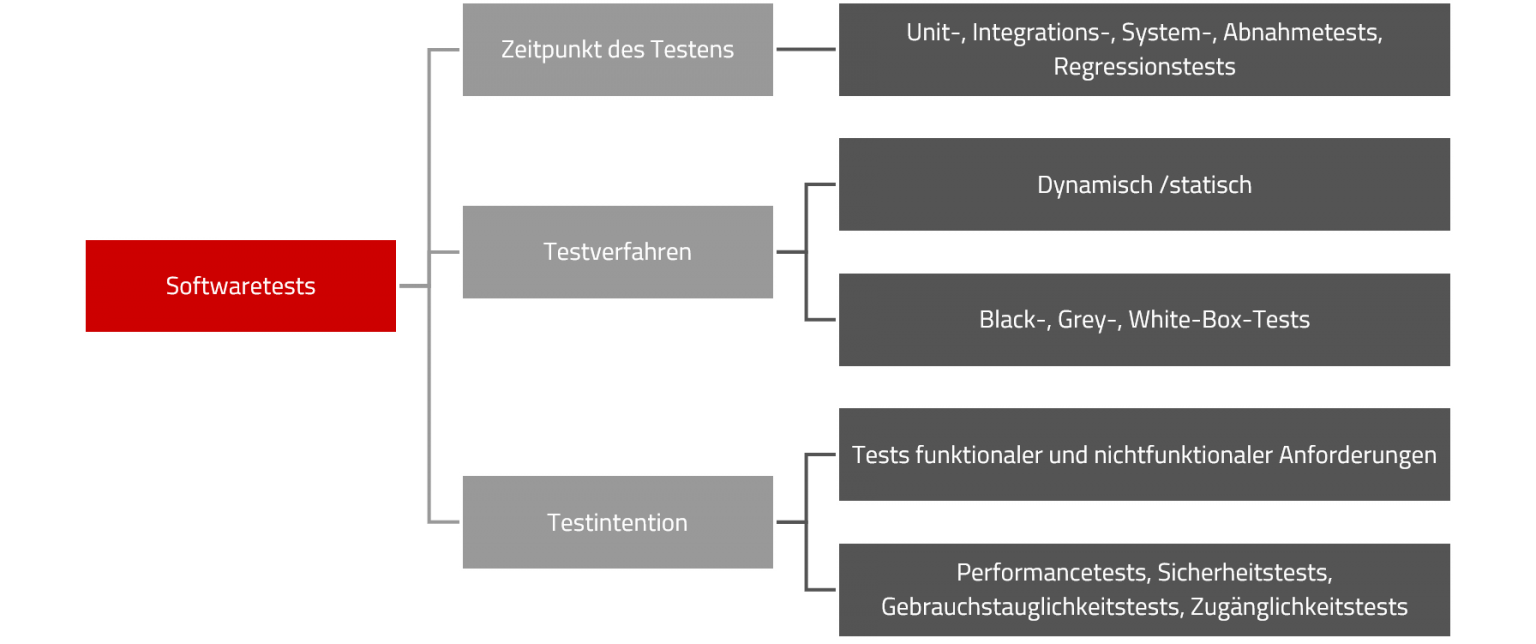
\includegraphics[scale=.32]{Bilder/TestsKlassifizierung.png}
	Quelle: redbots \cite{testKlassifizierung}
\end{center}
